\documentclass[a4paper, 12pt]{article}

\usepackage{/Users/zhengz/Desktop/Math/Workspace/Homework1/homework}
%%%%%%%%%%%%%%%%%%%%%%%%%%%%%%%%%%%%%%%%%%%%%%%%%%%%%%%%%%%%%%%%%%%%%%%%%%%%%%%%%%%%%%%%%%%%%%%%%%%%%%%%%%%%%%%%%%%%%%%%%%%%%%%%%%%%%%%%
\begin{document}
%Header-Make sure you update this information!!!!
\noindent
%%%%%%%%%%%%%%%%%%%%%%%%%%%%%%%%%%%%%%%%%%%%%%%%%%%%%%%%%%%%%%%%%%%%%%%%%%%%%%%%%%%%%%%%%%%%%%%%%%%%%%%%%%%%%%%%%%%%%%%%%%%%%%%%%%%%%%%%
\large\textbf{Zhengdong Zhang} \hfill \textbf{Homework 3}   \\
Email: zhengz@uoregon.edu \hfill ID: 952091294 \\
\normalsize Course: MATH 635 - Algebraic Topology II \hfill Term: Winter 2025\\
Instructor: Dr.Daniel Dugger \hfill Due Date: $30^{th}$ January, 2025 \\
\noindent\rule{7in}{2.8pt}
\setstretch{1.1}

%%%%%%%%%%%%%%%%%%%%%%%%%%%%%%%%%%%%%%%%%%%%%%%%%%%%%%%%%%%%%%%%%%%%%%%%%%%%%%%%%%%%%%%%%%%%%%%%%%%%%%%%%%%%%%%%%%%%%%%%%%%%%%%%%%%%%%%%
%Probelm 1
%%%%%%%%%%%%%%%%%%%%%%%%%%%%%%%%%%%%%%%%%%%%%%%%%%%%%%%%%%%%%%%%%%%%%%%%%%%%%%%%%%%%%%%%%%%%%%%%%%%%%%%%%%%%%%%%%%%%%%%%%%%%%%%%%%%%%%%%
\begin{problem}{1}
Let \(x\) be the basepoint of \(S^n\). Identify \(S^n\vee S^n\) with the subspace \((S^n\times \left\{ x \right\})\cup (\left\{ x \right\}\times S^n)\) of 
\(S^n\vee S^n\). Prove that the diagram 
\[\begin{tikzcd}
	{S^n} & {S^n\times S^n} \\
	& {S^n\vee S^n}
	\arrow["\Delta", from=1-1, to=1-2]
	\arrow["{\text{pinch}}"', from=1-1, to=2-2]
	\arrow["j"', tail, from=2-2, to=1-2]
\end{tikzcd}\]
commutes up to homotopy, where \(\Delta\) is the diagonal map and \(j\) is the inclusion. 
\end{problem}
\begin{solution}
Embed \(S^n\) into \(\mathbb{R}^{n+1}\) canonically with \(x_1^2+\cdots+x_n^2+x_{n+1}^2=1\). Choose coordinates properly such that \(x\) is on the equator \(x_{n+1}=0\). The pinch map \(S^n\rightarrow S^n\vee S^n\) collapses the equator \(\left\{ x_{n+1}=0 \right\}\) and 
sends \(\left\{ x_{n+1}\geq 0 \right\}\) to the first \(S^n\) in \(S^n\vee S^n\) and \(\left\{ x_{n+1}\leq 0 \right\}\) to the second \(S^n\vee S^n\). For any point \(y=(y_1,\ldots,y_{n+1})\in S^n\), if \(y_{n+1}>0\), then the composition 
\(S^n\xrightarrow{\text{pinch}}S^n\vee S^n\hookrightarrow S^n\times S^n\) sends \(y\) to the point \((y,x)\). If \(y_{n+1}<0\), it was sent to \((x,y)\). And if \(y_{n+1}=0\), the point \(y\) is on the equator and it was sent to 
\((x,x)\). Now we need to show that the diagonal map \(\Delta:S^n\rightarrow S^n\times S^n\) is homotopic to the inclusion map 
\begin{align*}
	i:S^n&\rightarrow S^n\times S^n,\\
	  y&\mapsto (y,x) 
\end{align*}
Since \(S^n\) is path-connected, there exists a continous path \(\gamma:I\rightarrow S^n\) such that \(\gamma(0)=x\) and \(\gamma(1)=y\). Define a map 
\begin{align*}
	H:S^n\times I&\rightarrow S^n\times S^n,\\ 
      (y,t)&\mapsto (y,\gamma(t)).
\end{align*}
\(H\) is continous since \(\gamma\) is continous. \(H(-,0)=i\) and \(H(-,1)=\Delta\). This proves that \(i\) is homotopic to \(\Delta\) and similarly, \(y\mapsto (x,y)\) is also homotopic to \(\Delta\). This proves that the diagram 
\[\begin{tikzcd}
	{S^n} & {S^n\times S^n} \\
	& {S^n\vee S^n}
	\arrow["\Delta", from=1-1, to=1-2]
	\arrow["{\text{pinch}}"', from=1-1, to=2-2]
	\arrow["j"', tail, from=2-2, to=1-2]
\end{tikzcd}\]
is commutative.
\end{solution}

\noindent\rule{7in}{2.8pt}
%%%%%%%%%%%%%%%%%%%%%%%%%%%%%%%%%%%%%%%%%%%%%%%%%%%%%%%%%%%%%%%%%%%%%%%%%%%%%%%%%%%%%%%%%%%%%%%%%%%%%%%%%%%%%%%%%%%%%%%%%%%%%%%%%%%%%%%%
%Probelm 2
%%%%%%%%%%%%%%%%%%%%%%%%%%%%%%%%%%%%%%%%%%%%%%%%%%%%%%%%%%%%%%%%%%%%%%%%%%%%%%%%%%%%%%%%%%%%%%%%%%%%%%%%%%%%%%%%%%%%%%%%%%%%%%%%%%%%%%%%
\begin{problem}{2}
Let \(X\) be a topological space with a continous map \(\mu:X\times X\rightarrow X\). Assume there is an element \(e\in X\) with the property that \(\mu(e,x)=\mu(x,e)=x\) for all 
\(x\in X\). Write \(x\cdot y\) for \(\mu(x,y)\).
\begin{enumerate}[(a)]
\item Prove that \(\pi_1(X,e)\) is abelian.
\item If \(f,g:(I^n,\partial I^n)\rightarrow (X,e)\), let \(f\diamond g:I^n\rightarrow X\) be given by \((f\diamond g)(a)=f(a)\cdot g(a)\). Prove that the \(\diamond\) defines a unital operation on \(\pi_n(X,e)\).
\item Prove this operation on \(\pi_n(X,e)\) agrees with the usual one (defined in class for any space \(X\)). That is, prove that if \(f,g\in \pi_n(X,e)\), then \(f*g=f\diamond g\). 
\end{enumerate}
\end{problem}
\begin{solution}
\begin{enumerate}[(a)]
\item 
First we prove a useful claim. 
\begin{claim}
Let \(f,g,h,k:(I^n,\partial I^n)\rightarrow (X,e)\) be continous maps. We have 
\[(f*g)\cdot (h*k)=(f\cdot h)*(g\cdot k).\]
\end{claim}
\begin{claimproof}
Recall by definition 
\[(f*g)(t)=\begin{cases}
	g(2t,y),&\iif 0\leq t\leq 1/2, y\in I^{n-1};\\
	f(2t-1,y),&\iif 1/2\leq t\leq 1, y\in I^{n-1}.
\end{cases}\ \ \ \text{and}\ \ \ (h*k)(t)=\begin{cases}
    k(2t,y),&\iif 0\leq t\leq 1/2, y\in I^{n-1};\\ 
	h(2t-1,y),&\iif 1/2\leq t\leq 1, y\in I^{n-1}.
\end{cases}\]
So \((f*g)\cdot (h*k)\) can be written as 
\[(f*g)\cdot (h*k)(t)=\begin{cases}
	g(2t,y)\cdot k(2t,y),&\iif 0\leq t\leq 1/2, y\in I^{n-1};\\ 
    f(2t-1,y)\cdot h(2t-1,y),&\iif 1/2\leq t\leq 1, y\in I^{n-1}.
\end{cases}\]
This is exactly the definition of \((f\cdot h)*(g\cdot k)\).
\end{claimproof}

We have already know that \(\pi_1(X,e)\) has a group structure with the homotopy class of the constant map \([C_e]\) represents the identity element. For any \(\beta:(I,\partial I)\rightarrow (X,e)\), we have 
\([C_e*\beta]=[\beta*C_e]\) in \(\pi_1(X,e)\). There exists a continous map 
\(H_1:I\times I\rightarrow X\) such that \(H_1(x,0)=\beta(x)*C_e\), \(H_1(x,1)=(C_e*\beta)(x)\) and \(H_1(0,t)=H_1(1,t)=e\) for all \(t\in I\). Similarly, for any \(\gamma:(I,\partial I)\rightarrow (X,e)\), there exists a continous map 
\(H_2:I\times I\rightarrow X\) such that \(H_2(x,0)=C_e*\gamma(x)\), \(H_2(x,1)=(\gamma(x)*C_e)\) and \(H_2(0,t)=H_2(1,t)=e\) for all \(t\in I\). We define a map 
\begin{align*}
	H:I&\times I\rightarrow X,\\
	(x,t)&\mapsto H_1(x,t)\cdot H_2(x,t).
\end{align*}
This map is continous since it is the composition 
\[I\times I\xrightarrow{(H_1,H_2)}X\times X\xrightarrow{\mu} X.\]
Moreover, note that by the claim 
\begin{align*}
	H(x,0)&=H_1(x,0)\cdot H_2(x,0)=(\beta(x)*C_e)\cdot(C_e*\gamma(x))=(\beta*\gamma)(x),\\ 
	H(x,1)&=H_1(x,1)\cdot H_2(x,1)=(C_e*\beta(x))\cdot(\gamma(x)*C_e)=(\gamma*\beta)(x).
\end{align*}
And for any \(t\in I\), we have \(H(0,t)=H(1,t)=H_1(0,t)\cdot H_2(0,t)=e\). Thus, we can conclude that \(\beta*\gamma\) and \(\gamma*\beta\) represents the same homotopy class in \(\pi_1(X,e)\), which means \(\pi_1(X,e)\) is abelian.
\item Let \(C_e:(I^n,\partial I)\rightarrow (X,e)\) be the constant map at the base point \(e\). For any map \(f:(I^n,\partial I^n)\rightarrow (X,e)\), we have 
\[(C_e\diamond f)(a)=(C_e)(a)\cdot f(a)=e\cdot f(a)=f(a)\]
for any \(a\in I\). Same for \(f\diamond C_e\). This shows that \(\diamond\) defines a unital operation on paths. 
\item Given two paths \(f,g:(I^n,\partial I^n)\rightarrow (X,e)\), use the claim in part (a) and note that \(C_e*f\) is homotopic to \(f\) and \(g*C_e\) is homotopic to \(g\), we have 
\begin{align*}
f\diamond g &\simeq (C_e*f)\diamond (g*C_e)\\ 
            &=(C_e\diamond g)*(f\diamond C_e)\\ 
			&=g*f\\ 
			&\simeq f*g.
\end{align*}
The last step is because \(\pi_n(X,e)\) is abelian for all \(n\geq 1\). We have proved \(f\diamond g=f*g\) in \(\pi_n(X,e)\).
\end{enumerate}
\end{solution}

\noindent\rule{7in}{2.8pt}
%%%%%%%%%%%%%%%%%%%%%%%%%%%%%%%%%%%%%%%%%%%%%%%%%%%%%%%%%%%%%%%%%%%%%%%%%%%%%%%%%%%%%%%%%%%%%%%%%%%%%%%%%%%%%%%%%%%%%%%%%%%%%%%%%%%%%%%%
%Probelm 3
%%%%%%%%%%%%%%%%%%%%%%%%%%%%%%%%%%%%%%%%%%%%%%%%%%%%%%%%%%%%%%%%%%%%%%%%%%%%%%%%%%%%%%%%%%%%%%%%%%%%%%%%%%%%%%%%%%%%%%%%%%%%%%%%%%%%%%%%
\begin{problem}
Each part below gives a pushout diagram in a specified category \(\mathcal{C}\). For each one, identify the pushout with something explicit and (usually) familiar. 
\begin{enumerate}[(a)]
\item \(\mathcal{C}=\mathcal{Ab}\) (the category of abelian groups), and the diagram is 
\[\begin{tikzcd}
	A & B \\
	0
	\arrow["f", from=1-1, to=1-2]
	\arrow[from=1-1, to=2-1]
\end{tikzcd}\]
\item \(\mathcal{C}=\mathcal{Top}\) (the category of topological spaces), \(A\) is a subspace of \(X\), and the diagram is 
\[\begin{tikzcd}
	A & X \\
	{\left\{*\right\}}
	\arrow[tail, from=1-1, to=1-2]
	\arrow[from=1-1, to=2-1]
\end{tikzcd}\]
\item \(\mathcal{C}=\mathcal{Grp}\) (the category of groups), \(H\) is a subgroup of \(G\), and the diagram is 
\[\begin{tikzcd}
	H & G \\
	{\left\{*\right\}}
	\arrow[tail, from=1-1, to=1-2]
	\arrow[from=1-1, to=2-1]
\end{tikzcd}\]
(note that the answer is not \(G/H\), this one is a little tricky).
\item \(\mathcal{C}=\mathcal{Ab}\) and the diagram is 
\[\begin{tikzcd}
	A & C \\
	{A\oplus B}
	\arrow["f", from=1-1, to=1-2]
	\arrow["{i_1}"', from=1-1, to=2-1]
\end{tikzcd}\]
where \(i_1\) is the standard inclusion of \(A\) into the first summand of \(A\oplus B\).
\item \(\mathcal{C}=\mathcal{Ab}\) and the diagram is 
\[\begin{tikzcd}
	{\mathbb{Z}} & {\mathbb{Z}} \\
	{\mathbb{Z}}
	\arrow["2", from=1-1, to=1-2]
	\arrow["2"', from=1-1, to=2-1]
\end{tikzcd}\]
where both maps are multiplication by \(2\).
\item \(\mathcal{C}=\mathcal{Ab}\) and the diagram is 
\[\begin{tikzcd}
	{\mathbb{Z}} & {\mathbb{Z}} \\
	{\mathbb{Z}/2 \mathbb{Z}}
	\arrow["3", from=1-1, to=1-2]
	\arrow["\pi"', from=1-1, to=2-1]
\end{tikzcd}\]
where \(\pi\) is the usual quotient map. 
\item \(\mathcal{C}=\mathcal{Top}\) and the diagram is 
\[\begin{tikzcd}
	{S^1} & {D^2} \\
	{S^1}
	\arrow[tail, from=1-1, to=1-2]
	\arrow["f"', from=1-1, to=2-1]
\end{tikzcd}\]
where the horizontal map is the inclusion and the vertical map is \(f(z)=z^2\) (where \(S^1\) is identified with the unit complex numbers).
\item Compare and construct the pushouts of 
\[\begin{tikzcd}
	{\left\{0\right\}} & {\mathbb{Z}} \\
	{\mathbb{Z}}
	\arrow[from=1-1, to=1-2]
	\arrow[from=1-1, to=2-1]
\end{tikzcd}\]
in the category \(\mathcal{Ab}\), the category \(\mathcal{Grp}\), and the category \(\mathcal{Top}\) (where all three objects in the pushout are given the discrete topology).
\end{enumerate}    
\end{problem}
\begin{solution}
We will use the following construction of pushout in different categories:
\[\begin{tikzcd}
	A & C \\
	B
	\arrow["g", from=1-1, to=1-2]
	\arrow["f"', from=1-1, to=2-1]
\end{tikzcd}\]
In \(\mathcal{Top}\), the pushout can be constructed as the disjoint union \(B\sqcup C/\sim\) where \(f(a)\sim g(a)\) for all \(a\in A\). Similarly, in \(\mathcal{Ab}\), the pushout can be constructed as 
\(B\oplus C/\sim\) where \((f(a),0)\sim (0,g(a))\) for all \(a\in A\).
\begin{enumerate}[(a)]
\item By construction, the pushout is isomorphic to \(B\oplus 0/(f(A)=0)\), which is just the cokernel of the map \(A\xrightarrow{f} B\). 
\item By construction, the pushout is isomorphic to \(X\sqcup \left\{ * \right\}/\sim\) where \(*\) is identified with the image of \(A\) in X. This is the same as the quotient space \(X/A\). 
\item This is a quotient group of \(G\) where every elements in the subgroup \(H\) is sent to \(1\). Consider 
\[N=\la ghg^{-1}\mid g\in G, h\in H\ra.\]
\(N\) is the smallest normal subgroup of \(G\) containing \(H\). Suppose \(P\) is the pushout of \(\left\{ 1 \right\}\leftarrow H\rightarrow G\) in \(\mathcal{Grp}\):
\[\begin{tikzcd}
	H & G \\
	1 & P
	\arrow[from=1-1, to=1-2]
	\arrow[from=1-1, to=2-1]
	\arrow["f", from=1-2, to=2-2]
	\arrow[from=2-1, to=2-2]
\end{tikzcd}\]
\(f(H)=\left\{ 1 \right\}\) implies \(f(N)=\left\{ 1 \right\}\). So \(P\cong G/N\). 
\item By construction, the pushout is isomorphic to \(A\oplus B\oplus C/\sim \) where \((a,0,0)\sim (0,f(a),0)\). This is the same as identifying \(A\) as its image in \(B\). So the pushout is given by 
\[\begin{tikzcd}
	A & C \\
	{A\oplus B} & {C\oplus B}
	\arrow["f", from=1-1, to=1-2]
	\arrow["{\text{icl}}"', from=1-1, to=2-1]
	\arrow["{\text{icl}}", from=1-2, to=2-2]
	\arrow["{(f,id)}"', from=2-1, to=2-2]
\end{tikzcd}\]
\item By construction, the pushout is isomorphic to the abelian group \(\mathbb{Z}\oplus \mathbb{Z}/(2,-2)\sim(0,0)\). This is the same as the group 
\(\la (1,0),(1,-1)\ra/\la 2(1,-1)\ra\cong \mathbb{Z}\oplus (\mathbb{Z}/2)\).
\item By construction, the pushout is isomorphic to the abelian group \((\mathbb{Z}/2)\oplus \mathbb{Z}/\sim\) where \((0,3)\) is identified with \((1,0)\). The second part is the abelian group \(\mathbb{Z}/6 \mathbb{Z}\) and 
the first part \(\mathbb{Z}/2 \mathbb{Z}\) is identifies with the order 2 subgroup. So the pushout is isomorphic to \(\mathbb{Z}/6 \mathbb{Z}\). 
\item This is a CW complex \(X\). Its 1-skeleton \(X_1\) is isomorphic to \(S^1\) and a 2-cell \(D^2\) is glued to \(X_1\) via a 2-sheeted covering map. This is exactly the CW complex structure for \(\mathbb{R}P^2\), so the pushout is isomorphic to \(\mathbb{R}P^2\). 
\item In \(\mathbb{Ab}\), the pushout by construction is isomorphic to \(\mathbb{Z}\oplus \mathbb{Z}/\left\{ 0 \right\}\cong \mathbb{Z}\oplus \mathbb{Z}\). In \(\mathcal{Grp}\), the pushout is isomorphic to the free product \(\mathbb{Z}*\mathbb{Z}\). In \(\mathcal{Top}\), the pushout is the wedge sum 
\(\mathbb{Z}\vee \mathbb{Z}\) glued at \(0\) with discrete topology.
\end{enumerate}
\end{solution}

\noindent\rule{7in}{2.8pt}
%%%%%%%%%%%%%%%%%%%%%%%%%%%%%%%%%%%%%%%%%%%%%%%%%%%%%%%%%%%%%%%%%%%%%%%%%%%%%%%%%%%%%%%%%%%%%%%%%%%%%%%%%%%%%%%%%%%%%%%%%%%%%%%%%%%%%%%%
%Probelm 4
%%%%%%%%%%%%%%%%%%%%%%%%%%%%%%%%%%%%%%%%%%%%%%%%%%%%%%%%%%%%%%%%%%%%%%%%%%%%%%%%%%%%%%%%%%%%%%%%%%%%%%%%%%%%%%%%%%%%%%%%%%%%%%%%%%%%%%%%
\begin{problem}{4}
Suppose you are told that the following three squares are pushout diagrams 
\[\begin{tikzcd}
	A & B & A & C & B & P \\
	C & P & {*} & X & {*} & Y
	\arrow[from=1-1, to=1-2]
	\arrow[from=1-1, to=2-1]
	\arrow[from=1-2, to=2-2]
	\arrow[from=1-3, to=1-4]
	\arrow[from=1-3, to=2-3]
	\arrow[from=1-4, to=2-4]
	\arrow[from=1-5, to=1-6]
	\arrow[from=1-5, to=2-5]
	\arrow[from=1-6, to=2-6]
	\arrow[from=2-1, to=2-2]
	\arrow[from=2-3, to=2-4]
	\arrow[from=2-5, to=2-6]
\end{tikzcd}\]
Prove that \(X\cong Y\). You can give the argument assuming you are in \(\mathcal{Top}\) if you want, or you can give it in any category with a terminal object \(*\); if you do the former, try to only use the categorical properties 
of pushouts and not anything special about topological spaces.
\end{problem}
\begin{solution}
We have the following commutative diagram 
\[\begin{tikzcd}
	A & B & {*} \\
	C & P & Y
	\arrow[from=1-1, to=1-2]
	\arrow[from=1-1, to=2-1]
	\arrow[from=1-2, to=1-3]
	\arrow[from=1-2, to=2-2]
	\arrow[from=1-3, to=2-3]
	\arrow[from=2-1, to=2-2]
	\arrow[from=2-2, to=2-3]
\end{tikzcd}\]
Note that by uniqueness of the terminal object \(*\), the composition of maps \(A\rightarrow B\rightarrow *\) is the same map as \(A\rightarrow *\), since \(X\) is the pushout of the diagram 
\(C\leftarrow A\rightarrow *\), there exists a unique map \(f:X\rightarrow Y\) such that the following diagram commutes 
\[\begin{tikzcd}
	A & B & {*} \\
	C & P & Y \\
	&& X
	\arrow[from=1-1, to=1-2]
	\arrow[from=1-1, to=2-1]
	\arrow[from=1-2, to=1-3]
	\arrow[from=1-2, to=2-2]
	\arrow[from=1-3, to=2-3]
	\arrow[curve={height=-18pt}, from=1-3, to=3-3]
	\arrow[from=2-1, to=2-2]
	\arrow[from=2-1, to=3-3]
	\arrow[from=2-2, to=2-3]
	\arrow["{\exists !f}", dashed, from=3-3, to=2-3]
\end{tikzcd}\]
Now consider the following diagram 
\[\begin{tikzcd}
	A & B \\
	C & P \\
	&& X
	\arrow[from=1-1, to=1-2]
	\arrow[from=1-1, to=2-1]
	\arrow[from=1-2, to=2-2]
	\arrow[curve={height=-12pt}, from=1-2, to=3-3]
	\arrow[from=2-1, to=2-2]
	\arrow[curve={height=12pt}, from=2-1, to=3-3]
	\arrow["{\exists !g}"', dashed, from=2-2, to=3-3]
\end{tikzcd}\]
where \(B\rightarrow X\) is just the composition \(B\rightarrow *\rightarrow X\). This is part of the previous diagram so it commutes. Since \(P\) is the pushout of the diagram 
\(C\leftarrow A\rightarrow B\), there exists a unique map \(g:P\rightarrow X\) such that the above diagram commutes. Now let \(Z\) be an object in this category together with two maps 
\(P\rightarrow Z\) and \(*\rightarrow Z\) such that the following diagram commutes 
\[\begin{tikzcd}
	B & {*} \\
	P & Z
	\arrow[from=1-1, to=1-2]
	\arrow[from=1-1, to=2-1]
	\arrow[from=1-2, to=2-2]
	\arrow[from=2-1, to=2-2]
\end{tikzcd}\]
Since \(Y\) is the pushout of \(P\leftarrow B\rightarrow *\), there exists a unique map \(h:Y\rightarrow Z\) such that the following diagram commutes 
\[\begin{tikzcd}
	B & {*} \\
	P & Y \\
	&& Z
	\arrow[from=1-1, to=1-2]
	\arrow[from=1-1, to=2-1]
	\arrow[from=1-2, to=2-2]
	\arrow[curve={height=-12pt}, from=1-2, to=3-3]
	\arrow[from=2-1, to=2-2]
	\arrow[curve={height=12pt}, from=2-1, to=3-3]
	\arrow["{\exists !h}"', dashed, from=2-2, to=3-3]
\end{tikzcd}\]
Now consider the following diagram 
\[\begin{tikzcd}
	B & {*} \\
	P & Y & Z & X
	\arrow[from=1-1, to=1-2]
	\arrow[from=1-1, to=2-1]
	\arrow[from=1-2, to=2-2]
	\arrow[curve={height=-12pt}, from=1-2, to=2-4]
	\arrow[from=2-1, to=2-2]
	\arrow["g"', curve={height=30pt}, from=2-1, to=2-4]
	\arrow["h", from=2-2, to=2-3]
	\arrow["f", curve={height=-12pt}, from=2-4, to=2-2]
	\arrow[dashed, from=2-4, to=2-3]
\end{tikzcd}\]
This just combines the previous diagram and we can define a map \(h\circ f:X\rightarrow Z\) to make the diagram commutes, it is unique because both \(f\) and \(h\) are unique. This proves 
\(X\) satisfies the universal property of the pushout diagram \(*\leftarrow B\rightarrow P\), and by uniqueness of the pushout, we have \(X\cong Y\).
\end{solution}

\noindent\rule{7in}{2.8pt}
%%%%%%%%%%%%%%%%%%%%%%%%%%%%%%%%%%%%%%%%%%%%%%%%%%%%%%%%%%%%%%%%%%%%%%%%%%%%%%%%%%%%%%%%%%%%%%%%%%%%%%%%%%%%%%%%%%%%%%%%%%%%%%%%%%%%%%%%
%Probelm 5
%%%%%%%%%%%%%%%%%%%%%%%%%%%%%%%%%%%%%%%%%%%%%%%%%%%%%%%%%%%%%%%%%%%%%%%%%%%%%%%%%%%%%%%%%%%%%%%%%%%%%%%%%%%%%%%%%%%%%%%%%%%%%%%%%%%%%%%%
\begin{problem}{5}
In this problem we continue our exploration of \(3\)-dimensional manifolds. The ones you know at this point are 
\[S^3, \mathbb{R}P^3, S^2\times S^1, T^g\times S^1, N_r\times S^1\]
where \(T^g\) is the genus \(g\) torus and \(N_r=\mathbb{R}P^2\#\cdots\# \mathbb{R}P^2\) (connected sum of \(r\) copies of \(\mathbb{R}P^2\)). 
\begin{enumerate}
\item Make a table showing the homology groups with \(\mathbb{Z}\)-coefficients, with \(\mathbb{Q}\)-coefficients, and with \(\mathbb{Z}/2\)-coefficients for each of these spaces. 
\item Let \(X\) be the quotient of the cube \(I\times I\times I\) in which one identifies each face with its opposite face via a clockwise 90 degree rotation. Compute the homology groups of \(X\) and prove that 
this 3-manifold is different from all the ones listed above. 
\end{enumerate}
\end{problem}
\begin{solution}
\begin{enumerate}[(a)]
\item Consider the standard CW complex structure for a \(n\)-sphere (\(n\geq 1\)): one 0-cell and one n-cell. The boundary map is 0 so it does not change with different coefficients. So for any module \(M\), we have 
\[H_i(S^n;M)=\begin{cases}
	M,&\ \ \ \iif i=0,n;\\ 
	0,&\ \ \ \text{otherwise}
\end{cases}\] 
For \(\mathbb{R}P^n\) with \(n\geq 2\), consider the CW complex structure with only one \(k\)-cell in each dimension \(k\leq n\). The attaching map is given by 2-sheeted covering and we can calculate the cellular complex (Hatcher, Chapter 2, Example 2.42): 
\begin{align*}
	0\rightarrow \mathbb{Z}\xrightarrow{2} \mathbb{Z}\xrightarrow{0}\cdots\xrightarrow{2}\mathbb{Z}\xrightarrow{0}\mathbb{Z}\rightarrow 0 & \ \ \ \iif n\ \text{even},\\ 
	0\rightarrow \mathbb{Z}\xrightarrow{0} \mathbb{Z}\xrightarrow{2}\cdots\xrightarrow{2}\mathbb{Z}\xrightarrow{0}\mathbb{Z}\rightarrow 0 & \ \ \ \iif n\ \text{odd}.
\end{align*}
With \(\mathbb{Z}/2\)-coefficients, every \(\mathbb{Z}\xrightarrow{2}\mathbb{Z}\) becomes the zero map. With \(\mathbb{Q}\)-coefficients, every \(\mathbb{Z}\xrightarrow{2}\mathbb{Z}\) map becomes an isomorphism (2 is invertible in \(\mathbb{Q}\)). For \(n=2,3\), we have 
\begin{multicols}{2}
\noindent
	\[H_i(\mathbb{R}P^2;\mathbb{Z})=\begin{cases}
	\mathbb{Z}/2,&\ \ \ \iif i=1;\\ 
	\mathbb{Z},&\ \ \ \iif i=0;\\ 
	0,&\ \ \ \text{otherwise}.
\end{cases}\]
\[H_i(\mathbb{R}P^3;\mathbb{Z})=\begin{cases}
	\mathbb{Z}/2,&\ \ \ \iif i=1;\\ 
	\mathbb{Z},&\ \ \ \iif i=0,3;\\
	0,&\ \ \ \text{otherwise}.
\end{cases}\]
\end{multicols}
\begin{multicols}{2}
\noindent 
\[H_i(\mathbb{R}P^2;\mathbb{Z}/2)=\begin{cases}
	\mathbb{Z}/2,&\ \ \ \iif i=0,1,2;\\ 
	0,&\ \ \ \text{otherwise}.
\end{cases}\]
\[H_i(\mathbb{R}P^3;\mathbb{Z}/2)=\begin{cases}
	\mathbb{Z}/2,&\ \ \ \iif i=0,1,2,3;\\ 
	0,&\ \ \ \text{otherwise}.
\end{cases}\]
\end{multicols}
\begin{multicols}{2}
\noindent
\[H_i(\mathbb{R}P^2;\mathbb{Q})=\begin{cases}
   \mathbb{Q},&\ \ \ \iif i=0;\\ 
   0,&\ \ \ \text{otherwise}.
\end{cases}\]
\[H_i(\mathbb{R}P^3;\mathbb{Q})=\begin{cases}
	\mathbb{Q},&\ \ \ \iif i=0,3;\\ 
	0,&\ \ \ \text{otherwise}.
\end{cases}\]
\end{multicols}
Now we consider the connected sum of tori and real projective space, we have already calculate in Homework 1 using the cellular structure and chain complex:
\[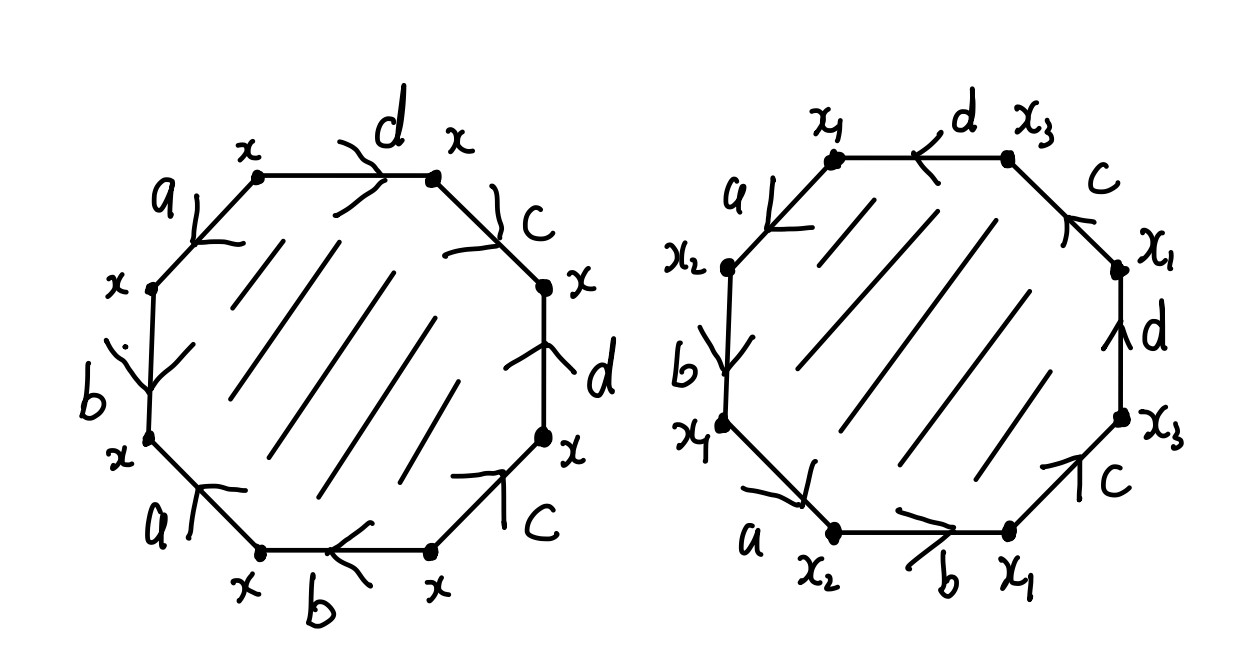
\includegraphics[scale=0.4]{Pictures/HW1-1-3.png}\]
\begin{align*}
	T^g:&\mathbb{Z}\xrightarrow{0}\mathbb{Z}^{2g}\xrightarrow{0}\mathbb{Z};\\ 
	N_r:&\mathbb{Z}\xrightarrow{d_2}\mathbb{Z}^{2r}\xrightarrow{d_1}\mathbb{Z}^{r+1}.
\end{align*} 
The cellular does not change with whatever coefficients we take. For \(N_r\), the boundary map is 
\[d_2(S)=2(a_1+b_1+\cdots+a_n+b_n)\]
where \(a_1,b_1,\ldots,a_n,b_n\) are 1-cells. So \(d_2=0\) in \(\mathbb{Z}/2\)-coefficients and \(d_2=(a_1+b_1+\cdots+a_n+b_n)\) with \(\mathbb{Q}\)-coefficients. \(d_1\) does not change. We summarize the homology as below. 
\begin{multicols}{2}
\noindent 
\[H_i(T^g;\mathbb{Z})=\begin{cases}
    \mathbb{Z},&\ \text{if}\ i=0,2;\\
    \mathbb{Z}^{2g},&\ \text{if}\ i=1;\\ 
    0,&\ \text{otherwise}. 
\end{cases}\]
\[H_i(N_r;\mathbb{Z})=\begin{cases}
    \mathbb{Z},&\ \text{if}\ i=0;\\ 
    \mathbb{Z}/2 \mathbb{Z}\oplus \mathbb{Z}^{r-1},&\ \text{if}\ i=1;\\ 
    0,&\ \text{otherwise}.
\end{cases}\]
\end{multicols}
\begin{multicols}{2}
\noindent 
\[H_i(T^g;\mathbb{Z}/2)=\begin{cases}
	\mathbb{Z}/2,&\ \iif\ i=0,2;\\ 
	(\mathbb{Z}/2)^{2g},&\ \iif \ i=1;\\ 
	0,&\ \text{otherwise}.
\end{cases}\]
\[H_i(N_r;\mathbb{Z}/2)=\begin{cases}
	\mathbb{Z}/2,&\ \ \iif\ i=0,2;\\ 
	(\mathbb{Z}/2)^r,&\ \ \iif i=1;\\ 
	0,&\ \ \text{otherwise}.
\end{cases}\]
\end{multicols}
\begin{multicols}{2}
\noindent 
\[H_i(T^g;\mathbb{Q})=\begin{cases}
	\mathbb{Q},&\ \iif \ i=0,2;\\ 
	(\mathbb{Q})^{2g},&\ \iif \ i=1;\\ 
	0,&\ \ \text{otherwise}.
\end{cases}\]
\[H_i(N_r;\mathbb{Q})=\begin{cases}
	\mathbb{Q},&\ \ \iif \ i=0;\\ 
	\mathbb{Q}^{r-1},&\ \ \iif\ i=1;\\ 
	0,&\ \ \text{otherwise}.
\end{cases}\]
\end{multicols}
Now to make the table for these 3-manifolds, use the fact that for any ring \(R\), 
\[H_n(X\times S^1;R)\cong H_n(X;R)\oplus H_{n-1}(X;R)\]
where \(X\) is a surface. 
\begin{table}[!h]
\begin{center}
\caption{Homology groups with \(\mathbb{Z}\)-coefficients}
\vspace{.1cm}
\begin{tabular}{|c||c|c|c|c|c|}
	\hline
	 & $H_*(S^3)$ & $H_*(\mathbb{R}P^3)$ & $H_*(S^2\times S^1)$ & $H_*(T^g\times S^1)$ & $ H_*(N_r\times S^1)$\\ 
	 \hline\hline
	0& $\mathbb{Z}$ & $\mathbb{Z}$ & \(\mathbb{Z}\) & \(\mathbb{Z}\) & \(\mathbb{Z}\) \\ 
	\hline
	1& \(0\) &  \(\mathbb{Z}/2 \mathbb{Z}\) & \(\mathbb{Z}\) & \(\mathbb{Z}^{2g+1}\) & \(\mathbb{Z}/2 \mathbb{Z} \oplus \mathbb{Z}^r\)\\ 
	\hline
	2& $0$   &   \(0\) & \(\mathbb{Z}\) & \(\mathbb{Z}^{2g+1}\) & \(\mathbb{Z}/2 \mathbb{Z}\oplus \mathbb{Z}^{r-1}\)\\ 
	\hline
	3& $\mathbb{Z}$ & $\mathbb{Z}$ & \(\mathbb{Z}\) & \(\mathbb{Z}\) & \(0\)\\
	\hline
\end{tabular}
\end{center}
\end{table}

\begin{table}[!h]
\begin{center}
\caption{Homology groups with \(\mathbb{Z}/2\)-coefficients}
\vspace{.1cm}
\begin{tabular}{|c||c|c|c|c|c|}
	\hline
	& $H_*(S^3)$ & $H_*(\mathbb{R}P^3)$ & $H_*(S^2\times S^1)$ & $H_*(T^g\times S^1)$ & $ H_*(N_r\times S^1)$\\ 
	\hline\hline 
	0&\(\mathbb{Z}/2\) & \(\mathbb{Z}/2\) & \(\mathbb{Z}/2\) & \(\mathbb{Z}/2\) & \(\mathbb{Z}/2\)\\ 
	\hline
	1&\(0\) & \(\mathbb{Z}/2\) & \(\mathbb{Z}/2\) & \((\mathbb{Z}/2)^{2g+1}\) & \((\mathbb{Z}/2)^{r+1}\) \\ 
	\hline
	2&\(0\) & \(\mathbb{Z}/2\) & \(\mathbb{Z}/2\) & \((\mathbb{Z}/2)^{2g+1}\) & \((\mathbb{Z}/2)^{r+1}\) \\ 
	\hline
	3&\(\mathbb{Z}/2\) & \(\mathbb{Z}/2\) & \(\mathbb{Z}/2\) & \(\mathbb{Z}/2\) & \((\mathbb{Z}/2)\) \\
	\hline
\end{tabular}
\end{center}
\end{table}

\begin{table}[!h]
	\begin{center}
	\caption{Homology groups with \(\mathbb{Q}\)-coefficients}
	\vspace{.1cm}
	\begin{tabular}{|c||c|c|c|c|c|}
		\hline
		& $H_*(S^3)$ & $H_*(\mathbb{R}P^3)$ & $H_*(S^2\times S^1)$ & $H_*(T^g\times S^1)$ & $ H_*(N_r\times S^1)$\\ 
		\hline\hline 
       0& \(\mathbb{Q}\) & \(\mathbb{Q}\) & \(\mathbb{Q}\) & \(\mathbb{Q}\) & \(\mathbb{Q}\) \\ 
	   \hline
	   1& \(0\) & \(0\) & \(\mathbb{Q}\) & \(\mathbb{Q}^{2g+1}\) & \(\mathbb{Q}^r\) \\ 
	   \hline
	   2& \(0\) & \(0\) & \(\mathbb{Q}\) & \(\mathbb{Q}^{2g+1}\) & \(\mathbb{Q}^{r-1}\) \\ 
	   \hline
	   3& \(\mathbb{Q}\) & \(\mathbb{Q}\) & \(\mathbb{Q}\) & \(\mathbb{Q}\) & \(0\) \\
       \hline
\end{tabular}
\end{center}
\end{table}
\item Let \(X\) be the described space. Consider the following cell complex structure
\[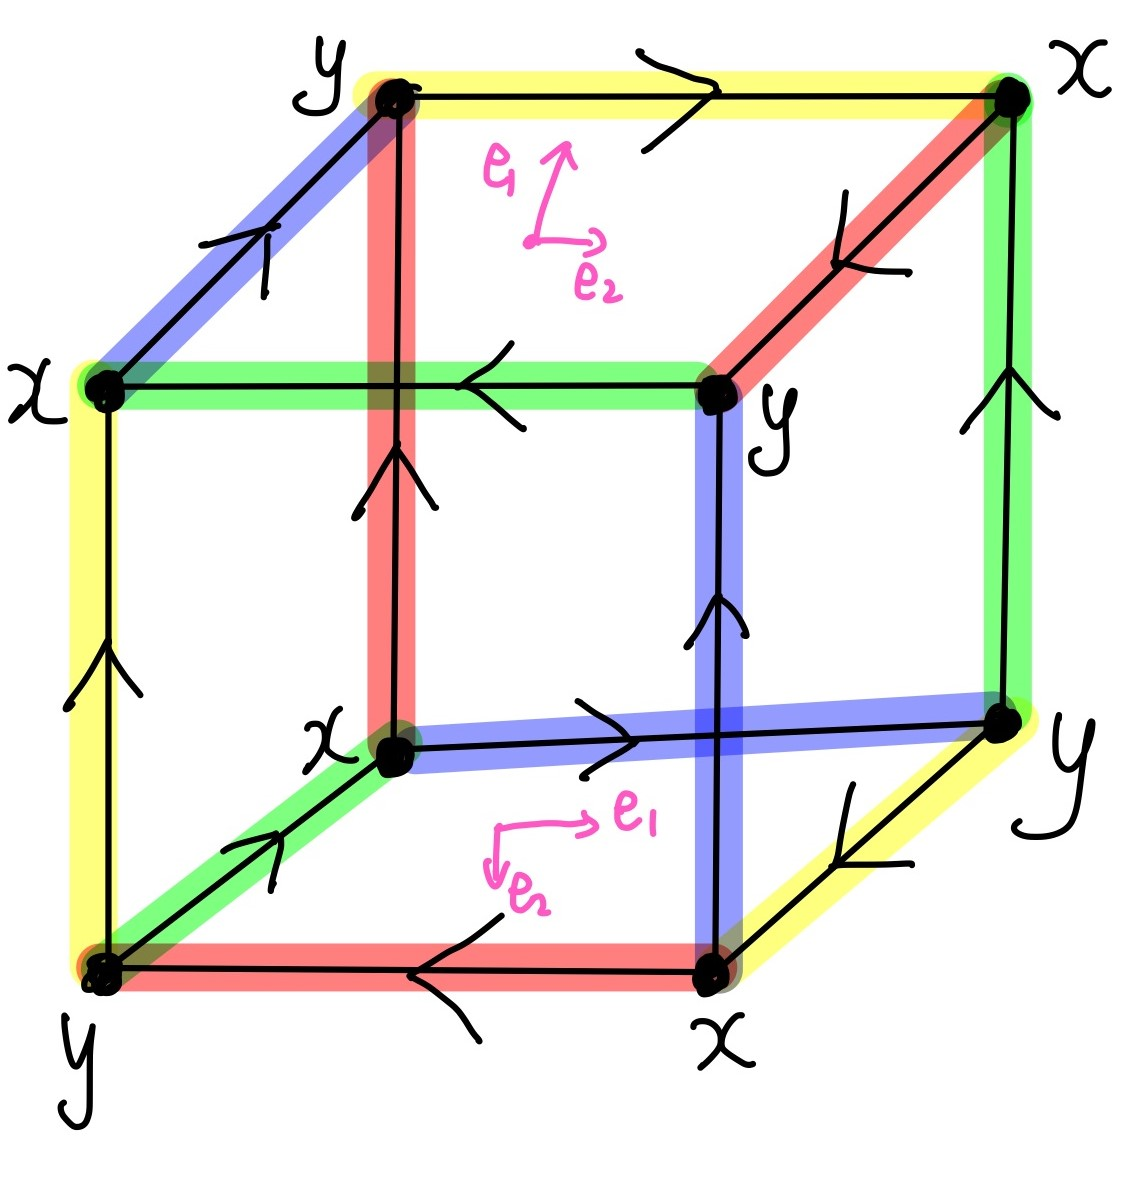
\includegraphics[scale=0.15]{Pictures/HW3-1.jpg}\] 
We have two 0-cells \(x\) and \(y\), four \(1\)-cells \(r,e,g,b\) (red, yellow, green, blue), three 2-cells \(T,F,S\) (Top, Front, Sides) and one 3-cell \(\Delta\). We have the following cellular complex: 
\[\mathbb{Z}\xrightarrow{d_3}\mathbb{Z}^3\xrightarrow{d_2}\mathbb{Z}^4\xrightarrow{ d_1}\mathbb{Z}^2\xrightarrow{d_0=0}0\]
For the boundary maps, we know that 
\[d_1(r)=d_1(b)=-d_1(g)=-d_1(e)=y-x\]
and 
\begin{align*}
	d_2(T)&=g+b+e+r,\\ 
	d_2(F)&=e+r-g-b,\\ 
	d_2(S)&=e+b-r-g.
\end{align*}
\begin{claim}
The boundary map \(d_3=0\).
\end{claim}
\begin{claimproof}
Consider the orientation (pink arrows on the top face) given at the point \(p\) by the ordered vector \(e_1,e_2\). This is the same as the ordered vector shown at the bottom face (twisted by how we glue the top and bottom faces). Consider the attaching 
map of 3-cells. We need to calculate the degree of \(S^2\cong\partial \Delta\rightarrow X_2/F,S\cong S^2 \). This is a two sheeted covering with the second part twisted by 90 degrees. The orientation on the top face, while moving along the boundary of the 3-cell, will give 
us the opposite orientation as shown in the picture on the bottom face. So the degree of the gluing map must be 0.
\end{claimproof}

To calculate the change of variables, we first do a change of basis. Let \(A=e+r\), \(B=g+b\) and \(C=r-b\). Note that \(\ker d_1\) can be generated by \(A,B,C\). And \(\im d_2\) can be written as 
\(\la A+B,A-B,A-B-2C \ra\). So 
\begin{align*}
	H_1(X)&=\ker d_1/\im d_2\\ 
	      &=\la A,B,C\ra/\la A+B,A-B,A-B-2C\ra\\ 
	      &=\la A-B,B,C\ra/\la 2B, A-B, 2C\ra\\ 
		  &=\la B,C\ra/\la 2B,2C\ra\\ 
		  &=\mathbb{Z}/2 \mathbb{Z}\oplus \mathbb{Z}/2 \mathbb{Z}.
\end{align*}
\(H_0(X)=H_3(X)=\mathbb{Z}\) since \(X\) is path-connected and \(d_3=0\). And 
\(H_2(X)=\ker d_2=0\). To summarize 
\[H_i(X)=\begin{cases}
	\mathbb{Z},&\ \ \ \iif i=0,3;\\ 
	\mathbb{Z}/2 \mathbb{Z}\oplus \mathbb{Z}/2 \mathbb{Z},&\ \ \ \iif i=1;\\ 
	0,&\ \ \ \iif \text{otherwise}.
\end{cases}\] 
This does not match any homology groups of spaces in the table above, so this space \(X\) is different from all the ones listed above. 
\end{enumerate}
\end{solution}

\noindent\rule{7in}{2.8pt}
%%%%%%%%%%%%%%%%%%%%%%%%%%%%%%%%%%%%%%%%%%%%%%%%%%%%%%%%%%%%%%%%%%%%%%%%%%%%%%%%%%%%%%%%%%%%%%%%%%%%%%%%%%%%%%%%%%%%%%%%%%%%%%%%%%%%%%%%
%Probelm 6
%%%%%%%%%%%%%%%%%%%%%%%%%%%%%%%%%%%%%%%%%%%%%%%%%%%%%%%%%%%%%%%%%%%%%%%%%%%%%%%%%%%%%%%%%%%%%%%%%%%%%%%%%%%%%%%%%%%%%%%%%%%%%%%%%%%%%%%%
\begin{problem}{6}
Conisder the \(3\)-manifold \(\mathbb{R}P^3\#\mathbb{R}P^3\). Construct two cofiber sequences \(S^2\hookrightarrow \mathbb{R}P^3\#\mathbb{R}P^3\rightarrow \mathbb{R}P^3\vee \mathbb{R}P^3\) and 
\(X\hookrightarrow \mathbb{R}P^3\#\mathbb{R}P^3\rightarrow \mathbb{R}P^3\) where \(X\simeq \mathbb{R}P^2\). Use these to compute \(H_*(\mathbb{R}P^3\#\mathbb{R}P^3)\).
\end{problem}
\begin{solution}
The solutions are divided into two parts. Part (1) we show that we have two cofiber sequence 
\begin{align*}
	S^2&\hookrightarrow \mathbb{R}P^3\#\mathbb{R}P^3\rightarrow \mathbb{R}P^3\vee \mathbb{R}P^3\\ 
	\mathbb{R}P^2&\hookrightarrow \mathbb{R}P^3\# \mathbb{R}P^3\rightarrow \mathbb{R}P^3.
\end{align*}
In part (2), we use these two cofiber sequence to calculate \(H_*(\mathbb{R}P^3\# \mathbb{R}P^3)\).
\begin{enumerate}[(1)]
\item The connected sum of two copies of \(\mathbb{R}P^3\) is constructed by first deleting one 3-cell from each \(\mathbb{R}P^3\), and then glue the boundary of the deleted 3-cells together. Their boundary 
is homeomorphic to \(S^2\). Collapsing the glued boundary in \(\mathbb{R}P^3\# \mathbb{R}P^3\) is the same as gluing two \(\mathbb{R}P^3\) together at one point. This gives us the cofiber sequence 
\[S^2\hookrightarrow \mathbb{R}P^3\#\mathbb{R}P^3\rightarrow \mathbb{R}P^3\vee \mathbb{R}P^3\]
Now consider \(\mathbb{R}P^3\) with the standard CW complex structure: one cell in each dimension 0,1,2, and 3. The 2-skeleton of \(\mathbb{R}P^3\) is isomorphic to \(\mathbb{R}P^2\). Identify \(\mathbb{R}P^2\) with the 2-skeleton 
in one copy of \(\mathbb{R}P^3\) in the connected sum. Collapsing this 2-skeleton in \(\mathbb{R}P^3\# \mathbb{R}P^3\) gives back one full copy of \(\mathbb{R}P^3\). So we have a cofiber sequence 
\[\mathbb{R}P^2\hookrightarrow \mathbb{R}P^3\# \mathbb{R}P^3\rightarrow \mathbb{R}P^3.\]
\item The cofiber sequence 
\[\mathbb{R}P^2\hookrightarrow \mathbb{R}P^3\# \mathbb{R}P^3\rightarrow \mathbb{R}P^3\]
induceds a long exact sequence in reduced homology 
\[\begin{tikzcd}
	& {\tilde{H}_*(\mathbb{R}P^2)} & {\tilde{H}_*(\mathbb{R}P^3\#\mathbb{R}P^3)} & {\tilde{H}_*(\mathbb{R}P^3)} \\
	3 & 0 & {?} & {\mathbb{Z}} \\
	2 & 0 & {?} & 0 \\
	1 & {\mathbb{Z}/2} & {?} & {\mathbb{Z}/2} \\
	0 & 0
	\arrow[from=2-2, to=2-3]
	\arrow[from=2-3, to=2-4]
	\arrow[from=2-4, to=3-2]
	\arrow[from=3-2, to=3-3]
	\arrow[from=3-3, to=3-4]
	\arrow[from=3-4, to=4-2]
	\arrow[from=4-2, to=4-3]
	\arrow[from=4-3, to=4-4]
	\arrow[from=4-4, to=5-2]
\end{tikzcd}\]
We can see that \(H_3(\mathbb{R}P^3\#\mathbb{R}P^3)\cong H_3(\mathbb{R}P^3)=\mathbb{Z}\) and \(H_2(\mathbb{R}P^3\# \mathbb{R}P^3)=0\). Another cofiber sequence 
\[S^2\hookrightarrow \mathbb{R}P^3\#\mathbb{R}P^3\rightarrow \mathbb{R}P^3\vee \mathbb{R}P^3\]
also induces a long exact sequence in reduced homology 
\[\begin{tikzcd}
	& {\tilde{H}_*(S^2)} & {\tilde{H}_*(\mathbb{R}P^3\#\mathbb{R}P^3)} & {\tilde{H}_*(\mathbb{R}P^3\vee \mathbb{R}P^3)} \\
	3 & 0 & {\mathbb{Z}} & {\mathbb{Z}\oplus \mathbb{Z}} \\
	2 & {\mathbb{Z}} & 0 & 0 \\
	1 & 0 & {?} & {\mathbb{Z}/2\oplus\mathbb{Z}/2} \\
	0 & 0
	\arrow[from=2-2, to=2-3]
	\arrow[from=2-3, to=2-4]
	\arrow[from=2-4, to=3-2]
	\arrow[from=3-2, to=3-3]
	\arrow[from=3-3, to=3-4]
	\arrow[from=3-4, to=4-2]
	\arrow[from=4-2, to=4-3]
	\arrow[from=4-3, to=4-4]
	\arrow[from=4-4, to=5-2]
\end{tikzcd}\]
By exactness, \(H_1(\mathbb{R}P^3\# \mathbb{R}P^3)=\mathbb{Z}/2\oplus \mathbb{Z}/2\). Moreover, \(\mathbb{R}P^3\# \mathbb{R}P^3\) is path-connected since \(\mathbb{R}P^3\) is path connected, so the homology of \(\mathbb{R}P^3\# \mathbb{R}P^3\) can be summarized 
\[H_i(\mathbb{R}P^3\# \mathbb{R}P^3)=\begin{cases}
	\mathbb{Z},&\ \ \ \iif i=0,3;\\ 
	\mathbb{Z}/2\oplus \mathbb{Z}/2,&\ \ \ \iif i=1;\\ 
	0,&\ \ \ \text{otherwise}.
\end{cases}\]
\end{enumerate} 
\end{solution}

\noindent\rule{7in}{2.8pt}
%%%%%%%%%%%%%%%%%%%%%%%%%%%%%%%%%%%%%%%%%%%%%%%%%%%%%%%%%%%%%%%%%%%%%%%%%%%%%%%%%%%%%%%%%%%%%%%%%%%%%%%%%%%%%%%%%%%%%%%%%%%%%%%%%%%%%%%%
%Probelm 7
%%%%%%%%%%%%%%%%%%%%%%%%%%%%%%%%%%%%%%%%%%%%%%%%%%%%%%%%%%%%%%%%%%%%%%%%%%%%%%%%%%%%%%%%%%%%%%%%%%%%%%%%%%%%%%%%%%%%%%%%%%%%%%%%%%%%%%%%
\begin{problem}{7}
Identify \(S^1\) with the unit complex numbers, and let \(\pi:\mathbb{C}-0\rightarrow S^1\) be the map \(\pi(z)=z/|z|\). For each \(c\in \mathbb{R}_{>0}\) let \(j_c:S^1\hookrightarrow \mathbb{C}\) be the map \(j_c(z)=cz\).\\ 
Let \(f(z)\) be a degree \(n\) polynomial with coefficients in \(\mathbb{C}\), and for convenience assume \(f\) is monic. Let \(K\) be a positive real number that is larger than the norms of all the roots of \(f(z)\). 
Note that if \(c>K\) then \(f\) maps \(j_c(S^1)\) into \(\mathbb{C}-0\), and so we may consider the composite \(\pi fj_c\); it is a map \(S^1\rightarrow S^1\). 
\begin{enumerate}[(a)]
\item If \(K<c<d\) prove that \(\deg (\pi fj_c)=\deg (\pi fj_d)\). 
\item Prove that if \(c\) is large enough then \(fj_c\) is homotopic to the map \(z\mapsto z^n\).
\item Conclude that if \(c>K\) then \(\deg (\pi fj_c)=n\).
\item In this last part we will prove the Fundamental Theorem of Algebra. Suppose \(f\) does not have any roots at all. Prove that \(\pi fj_1\) factors through a contractible space, and use this to deduce a contradiction. 
\end{enumerate}
\end{problem}
\begin{solution}
\begin{enumerate}[(a)]
\item Consider the annulus \(A=\left\{ z\in \mathbb{C}\mid c\leq |z|\leq d \right\}\). For any \(z\in A\), \(|f(z)|>0\) since \(c>K\). Define the following map 
\begin{align*}
	H:S^1\times I&\rightarrow S^1,\\ 
	(z,t)&\mapsto \pi f((1-t)cz+tdz)
\end{align*}
Note that for any \(0\leq t\leq 1\), \(((1-t)c+td)z\in A\). So \(f((1-t)cz+tdz)\in \mathbb{C}-0\). And \(H(z,0)=\pi fj_c\) and \(H(z,1)=\pi fj_d\). This proves that \(\pi fj_c\) is homotopic to 
\(\pi fj_d\). Thus, we have \(\deg \pi fj_c=\deg \pi fj_d\). 
\item Write \(g(z)=c^nz^n\). We first prove that \(fj_c\) is homotopic to \(g\). Consider following map 
\begin{align*}
	H:S^1\times I&\rightarrow \mathbb{C}-0,\\ 
	(z,t)&\mapsto g(z)+t(f(cz)-g(z)).
\end{align*}
Write \(fj_c(z)=f(cz)=c^nz^n+a_{n-1}c^{n-1}z^{n-1}+\cdots+a_0\). Note that for any \(0\leq t\leq 1\), by reverse triangle inequality, we have 
\begin{align*}
	|g(z)+t(f(cz)-g(z))|&=|c^nz^n+ta_{n-1}c^{n-1}z^{n-1}+\cdots+a_0|\\ 
	                    &\geq c^n|z^n|-c^{n-1}t|a_{n-1}z^{n-1}|-\cdots-|a_0|\\ 
						=h(c).
\end{align*}
View the last thing as a polynomial in \(c\) and since \(|z|=1\) is bounded, if \(c\) is large enough, \(h(c)>0\). So we can choose a large \(c\) such that \(H\) is well-defined as the image lies in 
\(\mathbb{C}-0\). 

What remains to show is that for a large enough real constant \(M\), the map \(z\mapsto (cz)^n\) is homotopic to \(z\mapsto z^n\) on \(S^1=\left\{ |z|=1 \right\}\). Consider the homotopy 
\begin{align*}
	H:S^1\times I&\rightarrow \mathbb{C}-0,\\ 
	 (z,t)&\mapsto ((1-t)z+ctz)^n.
\end{align*}
This homotopy is well-defined since the only \(|z|=1\) implies \(|z^n|\neq 0\).
\item We need to show that \(p:S^1\rightarrow S^1\) by sending \(z\) to \(\frac{z^n}{|z^n|}\) has degree \(n\). Write \(z=e^{2\pi it}\) for \(0\leq t\leq 1\). We have 
\[p(z)=\frac{z^n}{|z^n|}=\frac{e^{2\pi nit}}{|e^{2\pi nit}|}=e^{2\pi nit}.\]
It is easy to see that \(p\) is just the \(n\) times counterclockwise rotation on \(S^1\). So \(\deg (p)=\deg (\pi fj_c)=n\).
\item Suppose \(f\) has no root at all. Then for any \(z\in \mathbb{C}\), the map \(\frac{f(z)}{|f(z)|}\) is continous and well-defined and \(f(z)\neq 0\). So we have a commutative diagram 
\[\begin{tikzcd}
	{S^1} && {S^1} \\
	{\mathbb{C}}
	\arrow["{\pi f(z)=\frac{f(z)}{|f(z)|}}", from=1-1, to=1-3]
	\arrow[hook', from=1-1, to=2-1]
	\arrow["{\frac{f(z)}{|f(z)|}}"', from=2-1, to=1-3]
\end{tikzcd}\]
This induces a map in homology 
\[\begin{tikzcd}
	{H_1(S^1)} && {H_1(S^1)} \\
	{H_1(\mathbb{C})}
	\arrow["{(\pi f)_*}", from=1-1, to=1-3]
	\arrow[hook', from=1-1, to=2-1]
	\arrow[from=2-1, to=1-3]
\end{tikzcd}\]
And since \(\mathbb{C}\) is contractible, \(H_1(\mathbb{C})=0\), so \((\pi f)_*\) is the zero map. We have \(\deg(\pi fj_1)=0\). But \(\deg(\pi fj_1)=n\) according to our previous discussion. A contradiction. \(f\) must 
have at least one root in \(\mathbb{C}\).
\end{enumerate}
\end{solution}

\end{document}